\chapter{実験と結果}	
\thispagestyle{plain}   % chapterの直後に必ず指定

\section{タスクの提示や会話機能の動作テスト}\label{sec:gpt_res_test}
この節では\ref{sec:gpt_res}節で開発した{\mason}のサバイバルモードのプレイヤー向けの対話機能について、目標を設定し動作テストの結果を述べる.

今回は{\mason}に表\ref{tab:goal_and_action}の目標や使用できる行動を設定し、{\mason}との対話機能を使用した。

\begin{table}[H]
    \caption{実験1の設定}\label{tab:goal_and_action}
    \centering
    \begin{tabular}{ll}
        \hline \hline
        目標 & ダイヤモンドを集める. \\
        \hline
        許可した行動 & mine\_block \\
          & craft\_item \\
        \hline
    \end{tabular}
\end{table}

目標への最序盤での対話の結果を図\ref{fig:first_task}に示す。
図を見ると、{\mason}はプレイヤーが森バイオームに位置し何も装備していないことなどからゲームの序盤であることを推論し、Minecraftの最も基本的な資源の木を集めるべきであるとタスクを提示している。
また、``木を集める''というタスクは{\mason}も行うことが出来るタスクであるためこの作業を手伝うかの提案を行っている。

\begin{figure}[H]
    \centering
    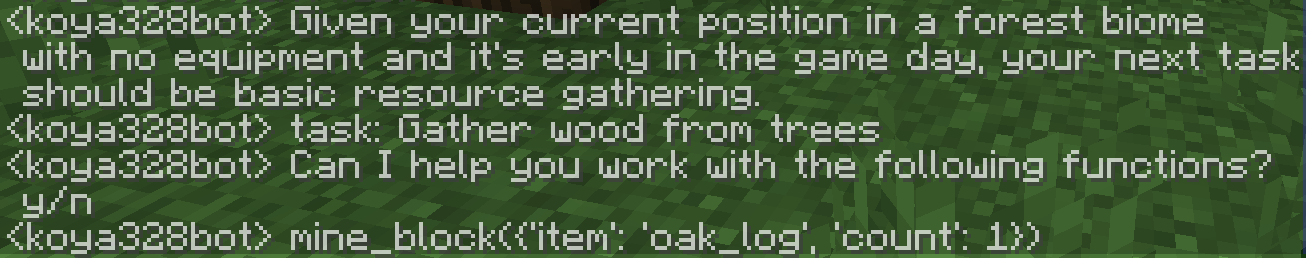
\includegraphics[width=0.95\textwidth]{fig/first_task.PNG}
    \caption{序盤のタスクの提示}
    \label{fig:first_task}
\end{figure}

木を切るタスクを手伝ってもらうために``y''で返答することで、図\ref{fig:task_help}のようにプレイヤーに提示したタスクを{\mason}も行うことが出来ている。
\begin{figure}[H]
    \centering
    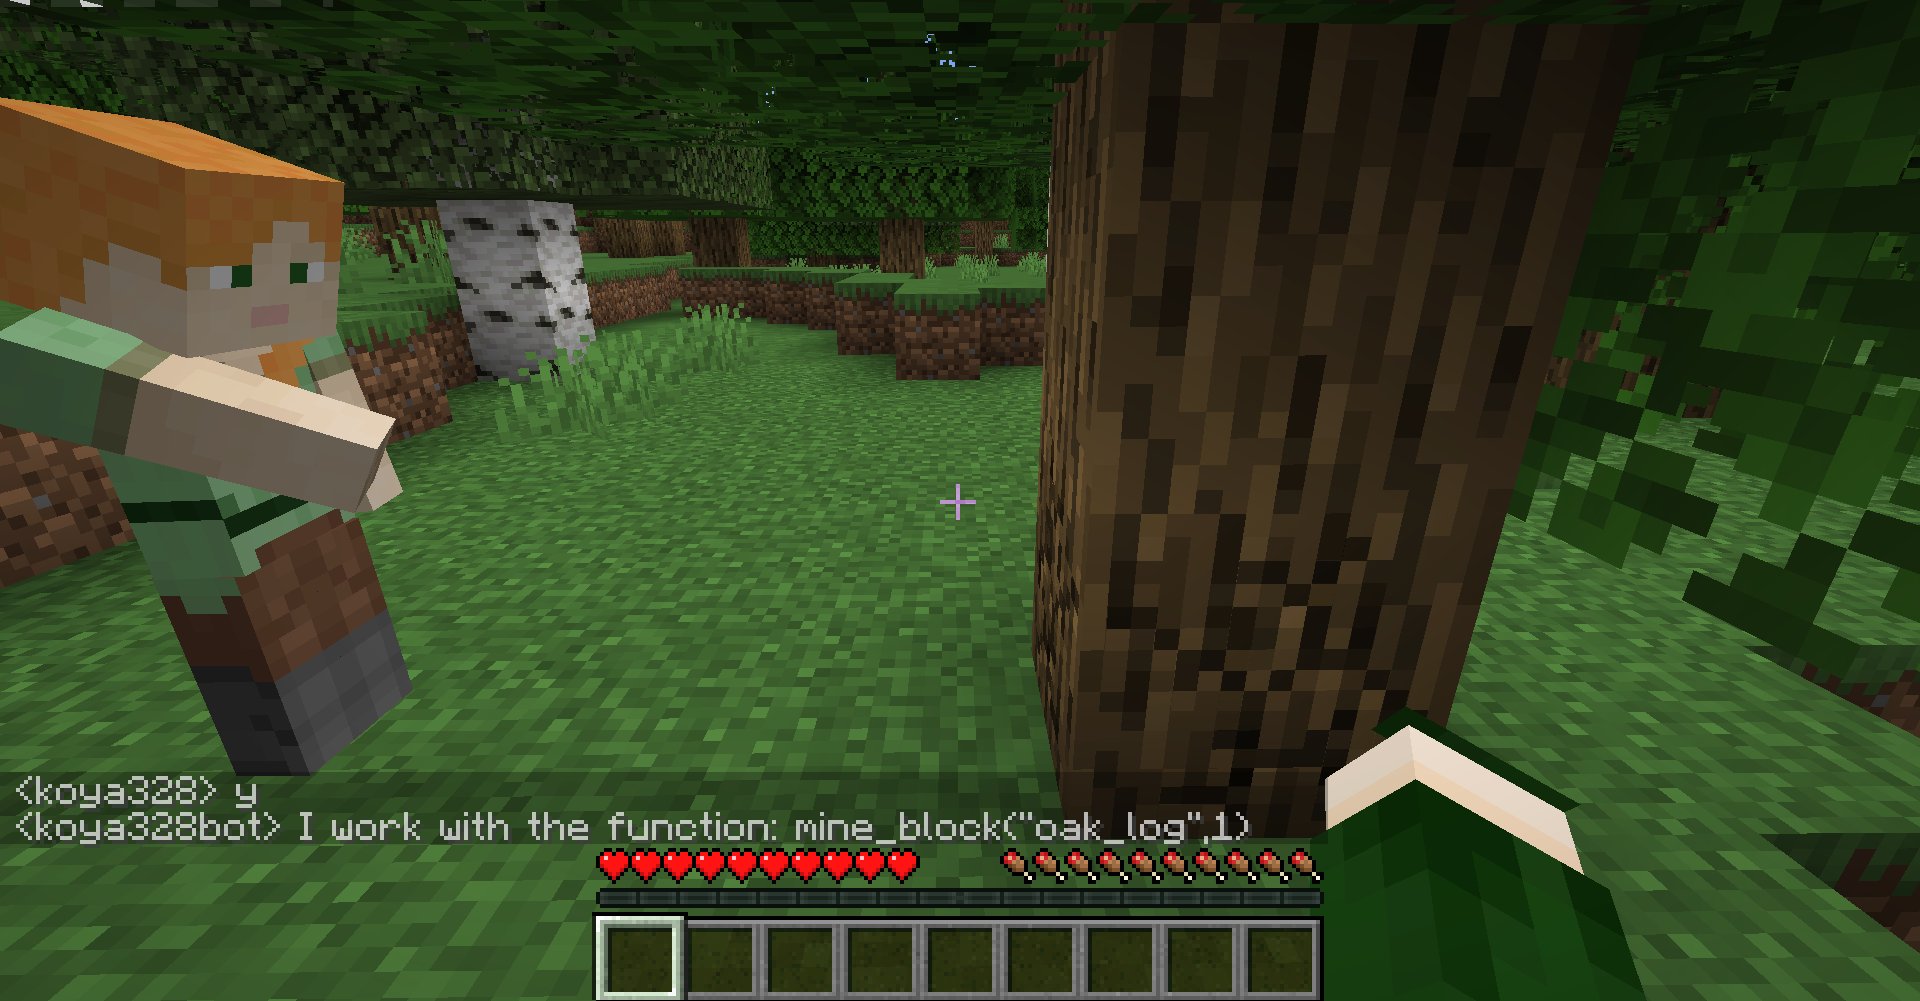
\includegraphics[width=0.95\textwidth]{fig/task_help.PNG}
    \caption{木を切る作業の支援}
    \label{fig:task_help}
\end{figure}

{\mason}はプレイヤーから話しかけられなくても定期的にタスクを提示することができ、木を切った後に図\ref{fig:wooden_pickaxe}のように木のピッケルを作るべきだというタスクを提示している。
木のピッケルの作り方がわからないプレイヤーが作り方を質問した場合、その質問に回答することが可能だった。
\begin{figure}[H]
    \centering
    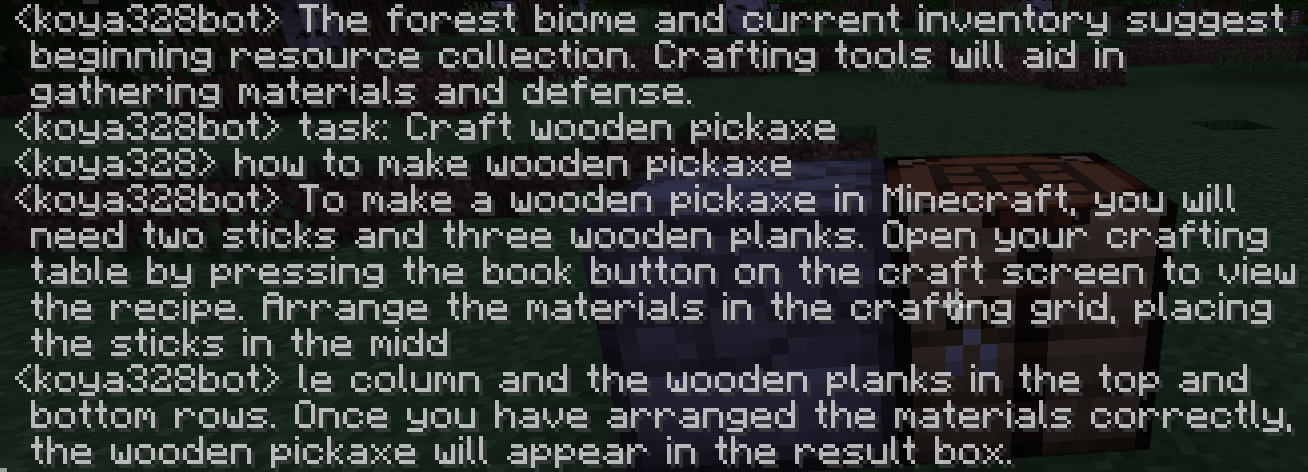
\includegraphics[width=0.95\textwidth]{fig/wooden_pickaxe.png}
    \caption{木を切る作業の支援}
    \label{fig:wooden_pickaxe}
\end{figure}

また、目標の達成とは関係ない質問 (図\ref{fig:diamond_question}はダイヤモンドを取得したあと何のアイテムを作ることが出来るかの質問)についても回答することが出来る。
\begin{figure}[H]
    \centering
    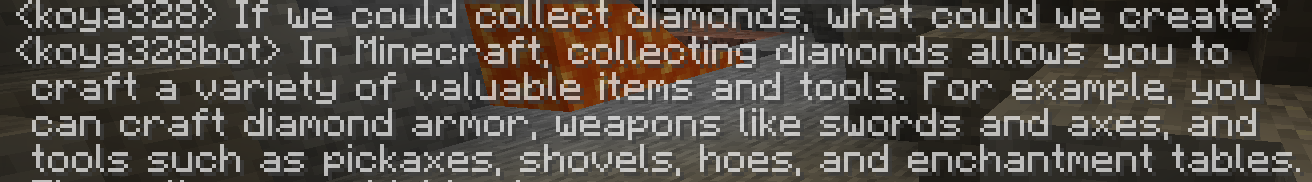
\includegraphics[width=0.95\textwidth]{fig/diamond_question.PNG}
    \caption{目標と関係ない質問をしたときの対話}
    \label{fig:diamond_question}
\end{figure}

目標の最終盤での対話の結果を図\ref{fig:final_task}に示す。
図を見ると、{\mason}はプレイヤー鉄のピッケルを持っていることからダイヤを採掘するタスクを提示出来ている。

\begin{figure}[H]
    \centering
    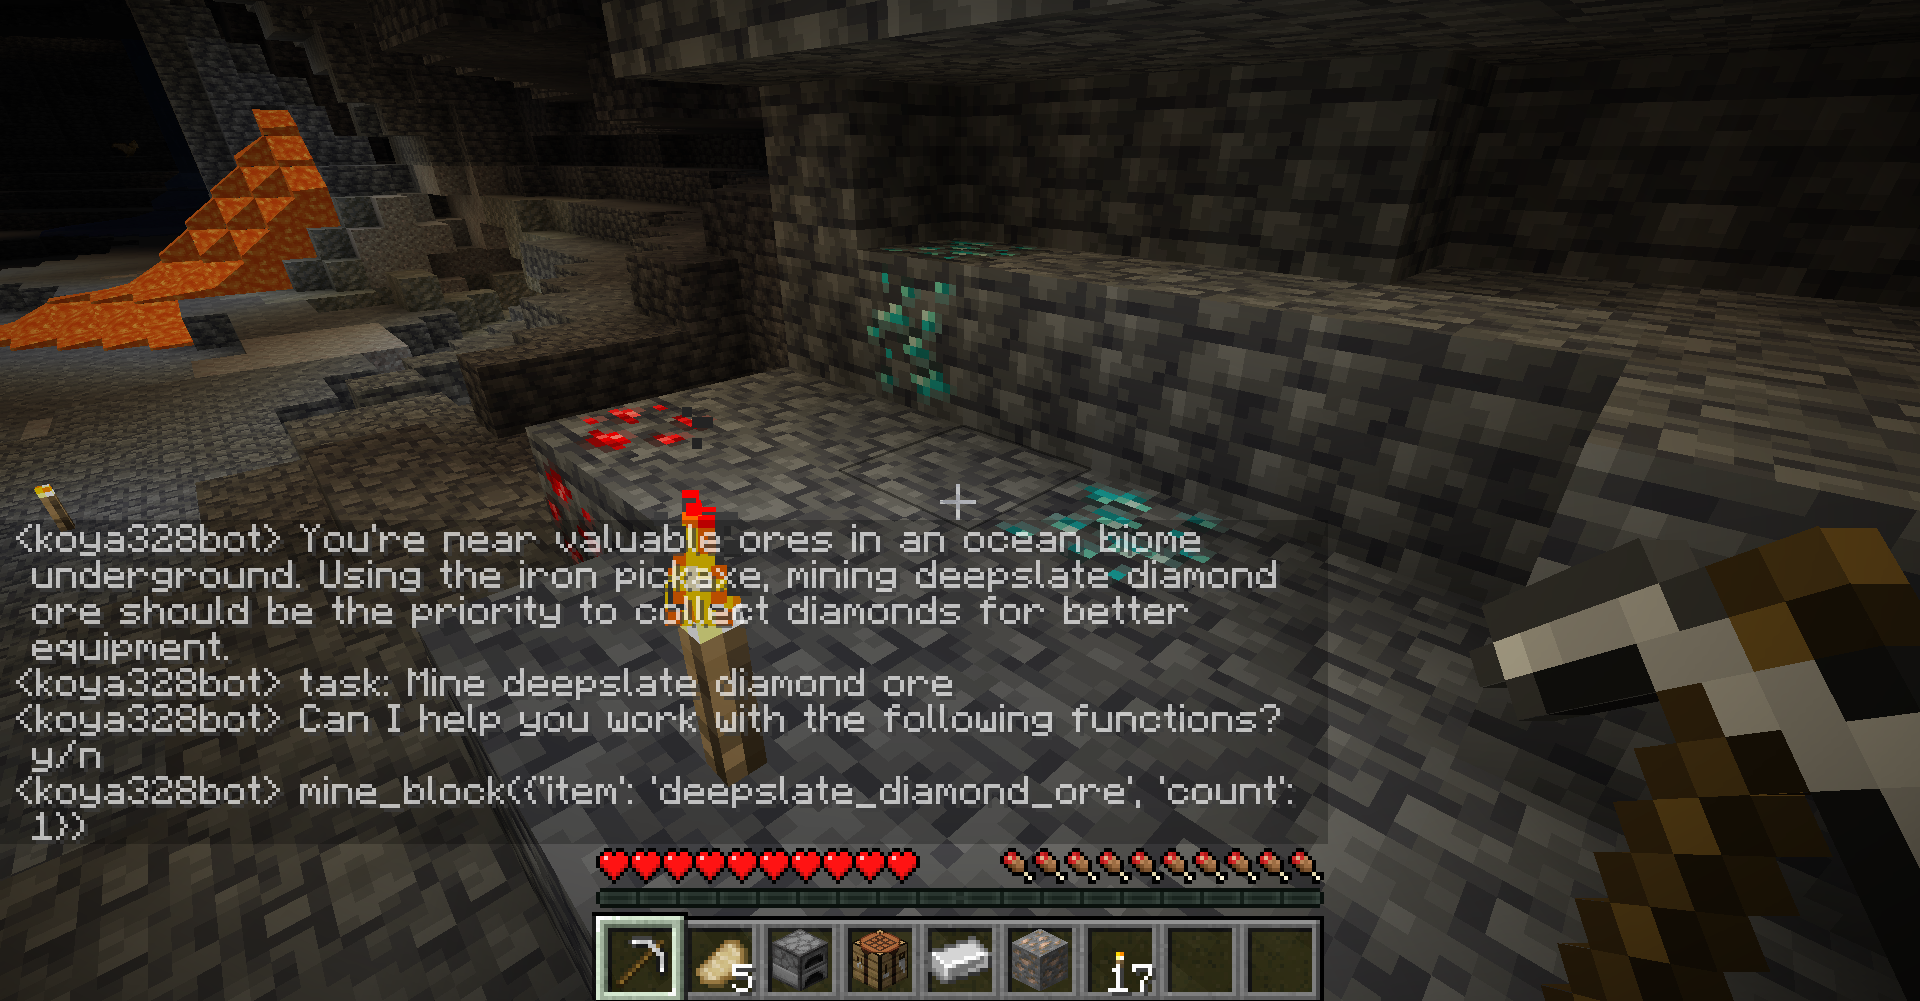
\includegraphics[width=0.95\textwidth]{fig/final_task.png}
    \caption{ダイヤモンド採掘の提示}
    \label{fig:final_task}
\end{figure}

\section{構造物自動生成の実験}\label{sec:build_mode_generate}
この節では,\ref{sec:build_mode}節にて解説したクリエイティブモード向け構造物自動生成機能がどのような構造物を生成可能であるかを,モデルやプロンプトの設定を踏まえて紹介する.

\subsection{実験1}\label{sec:ex1}
実験1では,{\mason}の自動生成機能において,詳細度の異なる2つのプロンプトをそれぞれ送信し,出力結果の比較を行った.今回の実験の設定内容は表\ref{tab:setting1}に記す.
今回のテストケースとして駅の構造を生成した.
なお,大規模言語モデルによる出力結果は一定ではないため,表\ref{tab:setting1}のとおり,それぞれのプロンプトを3度送信した.
その中から,それぞれ最も優れた結果を図\ref{fig:station1}に示す.
\begin{table}[H]
    \caption{実験1の設定}\label{tab:setting1}
    \centering
    \begin{tabular}{ll}
        \hline \hline
        モデル & gpt-3.5-turbo \\
        \hline
        左図プロンプト & train station \\
        \hline
        右図プロンプト & Build a train station.I want the tracks to use rails. \\
          & And build the platform well. \\
        \hline
        試行回数 & 3回 \\
        \hline
    \end{tabular}
\end{table}

\begin{figure}[H]
    \centering
    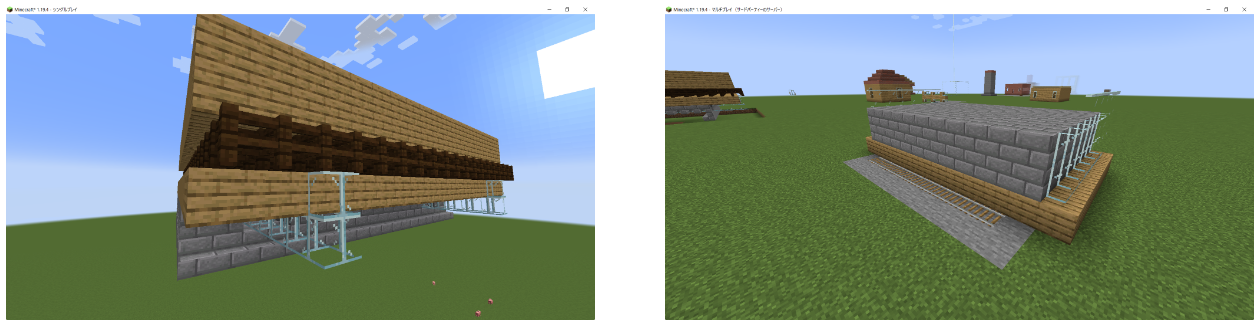
\includegraphics[width=0.95\textwidth]{fig/train_station1.PNG}
    \caption{実験1の生成結果}
    \label{fig:station1}
\end{figure}

図\ref{fig:station1}右図の出力結果を見ると駅の外装のような構造物を作成していることが示唆される.
しかし,左図構造物生成時のログを参照すると,下部の石レンガはプラットフォーム,上部の板材,ダークオークのフェンス,ガラスパネルはチケットカウンター,ベンチ,標識であると記載されているため,この出力結果は駅の外装ではなくモデルがあまり駅のプラットフォームについて理解せず生成したものであると言える.
右図では,ログを参照したところ板材と石レンガでプラットフォームを作り,それに沿うようにレールを敷いていると記載されているため,プロンプトによって出力改善されたことが分かる.

\subsection{実験2}\label{sec:ex2}
実験2では,{\mason}の自動生成機能において,詳細度の異なる2つのプロンプトをそれぞれ送信し,出力結果の比較を行った.今回の実験の設定内容は表\ref{tab:setting2}に記す.
実験1と同様に今回のテストケースとして駅の構造を生成した.
なお,大規模言語モデルによる出力結果は一定ではないため,表\ref{tab:setting2}のとおり,それぞれのプロンプトを3度送信した.
その中から,それぞれ最も優れた結果を図\ref{fig:station2}に示す.
\begin{table}[H]
    \caption{実験2の設定}\label{tab:setting2}
    \centering
    \begin{tabular}{ll}
        \hline \hline
        モデル & gpt-4 \\
        \hline
        左図プロンプト & train station \\
        \hline
        右図プロンプト & Build a train station.I want the tracks to use rails. \\
          & And build the platform well. \\
        \hline
        試行回数 & 3回 \\
        \hline
    \end{tabular}
\end{table}

\begin{figure}[H]
    \centering
    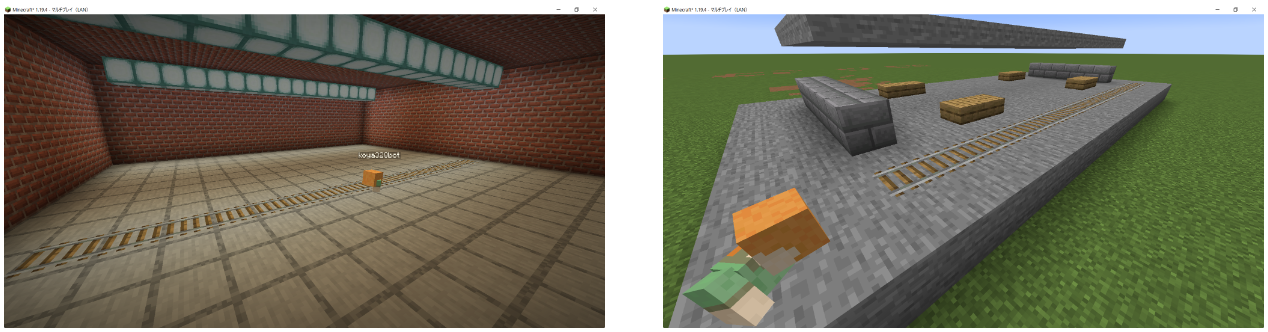
\includegraphics[width=0.95\textwidth]{fig/train_station2.PNG}
    \caption{実験2の生成結果}
    \label{fig:station2}
\end{figure}

\subsection{実験3}\label{sec:ex3}
実験3では,{\mason}の自動生成機能において,プロンプトによる構造物の生成を行い,その後追加のプロンプトを送信し,出力結果がどのように変化するかを検証した.今回の実験の設定内容は表\ref{tab:setting3}に記す.
今回のテストケースとしてまず家を作成するプロンプト(表\ref{tab:setting3}プロンプト1)を送信し,その後窓を追加するプロンプト(表\ref{tab:setting3}プロンプト2)を送信した.
なお,大規模言語モデルによる出力結果は一定ではないため,表\ref{tab:setting3}のとおり,プロンプトを3度送信し,その中から,最も優れた結果を図\ref{fig:add_window}に示す.

\begin{table}[H]
    \caption{実験3の設定}\label{tab:setting3}
    \centering
    \begin{tabular}{ll}
        \hline \hline
        モデル & gpt-4-1106-preview (GPT-4-Turbo) \\
        \hline
        プロンプト1 & please make house. \\
        \hline
        プロンプト2 & please add window. \\
        \hline
        試行回数 & 3回 \\
        \hline
    \end{tabular}
\end{table}

\begin{figure}[H]
    \centering
    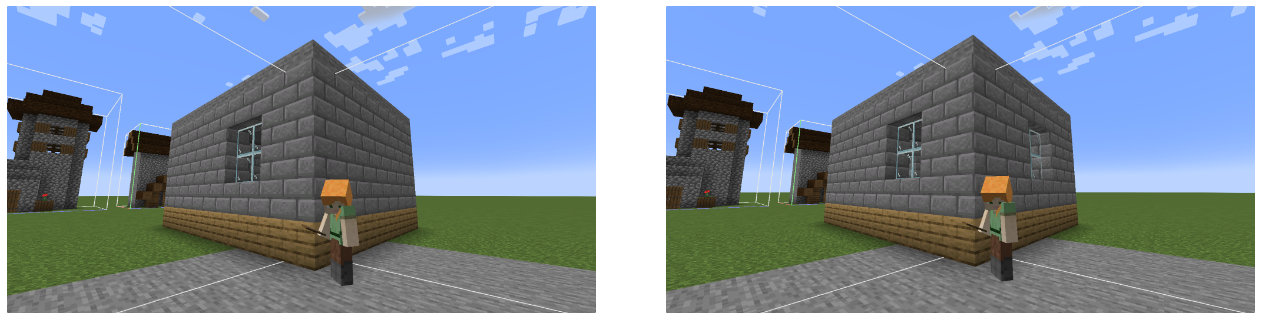
\includegraphics[width=0.95\textwidth]{fig/add_window.PNG}
    \caption{実験3の生成結果}
    \label{fig:add_window}
\end{figure}

\subsection{実験4}\label{sec:ex4}
実験4では,{\mason}の自動生成機能において,プロンプトによる構造物の生成を行い,その後追加のプロンプトを送信し,出力結果がどのように変化するかを検証した.今回の実験の設定内容は表\ref{tab:setting4}に記す.
実験3と同様にテストケースとしてまず家を作成するプロンプト(表\ref{tab:setting4}プロンプト1)を送信し,その後窓を追加するプロンプト(表\ref{tab:setting4}プロンプト2)を送信した.
なお,大規模言語モデルによる出力結果は一定ではないため,表\ref{tab:setting4}のとおり,プロンプトを3度送信し,その中から,最も優れた結果を図\ref{fig:add_window2}に示す.

\begin{table}[H]
    \caption{実験4の設定}\label{tab:setting4}
    \centering
    \begin{tabular}{ll}
        \hline \hline
        モデル & gpt-3.5-turbo-1106ファインチューニング済みモデル \\
        \hline
        プロンプト1 & please make house. \\
        \hline
        プロンプト2 & please add window. \\
        \hline
        試行回数 & 3回 \\
        \hline
    \end{tabular}
\end{table}

\begin{figure}[H]
    \centering
    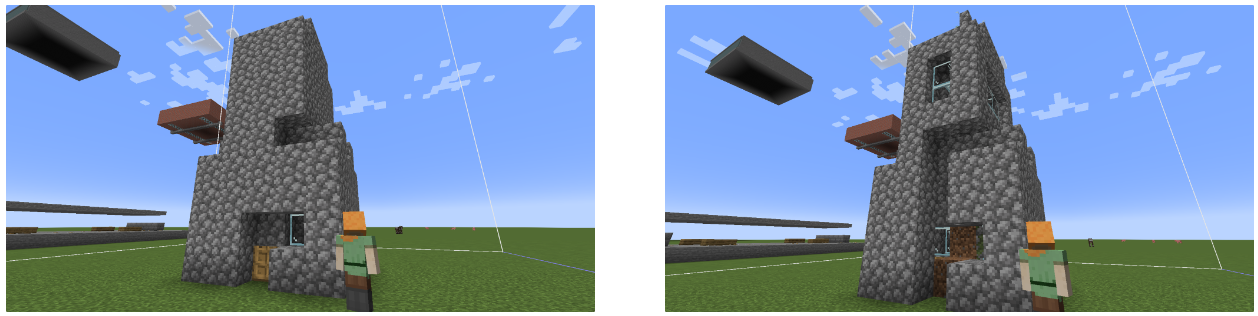
\includegraphics[width=0.95\textwidth]{fig/add_window2.PNG}
    \caption{実験3の生成結果}
    \label{fig:add_window2}
\end{figure}

\section{アンケートの実施と結果}\label{sec:survey_result}
botの有用性を検証するためbotのデモとアンケートを実施した.
デモ・アンケートは2023年10月16日に開催された,公立はこだて未来大学オープンラボの,イアンフランク研ブースにて行われ,計16人の学生がデモを行いアンケートに回答した.
デモではbotとの会話を始めに体験していただき,その後,ビルドモードを体験するように促した.

デモを行った後のアンケートの結果の一例について表\ref{tab:answer1},表\ref{tab:answer2}に示す.

``このbotを使うことで新しい建築のアイデアやインスピレーションを得ることができましたか?''という質問について,``そう思う''を4,``どちらかというとそう思う''を3,``どちらかというとそう思わない''を2,``そう思わない''を1として平均を計算した結果,3.2 となった.
表\ref{tab:answer1}の結果では肯定的な意見が得られているものの,表\ref{tab:answer2}の結果より平均が低いことや\ref{sec:build_mode_generate}節の生成結果から考察するとビルドモードは改善の必要があると考えられる.
\begin{table}[H]
    \centering
    \caption{このbotを使うことで新しい建築のアイデアやインスピレーションを得ることができましたか?}
    \label{tab:answer1}
    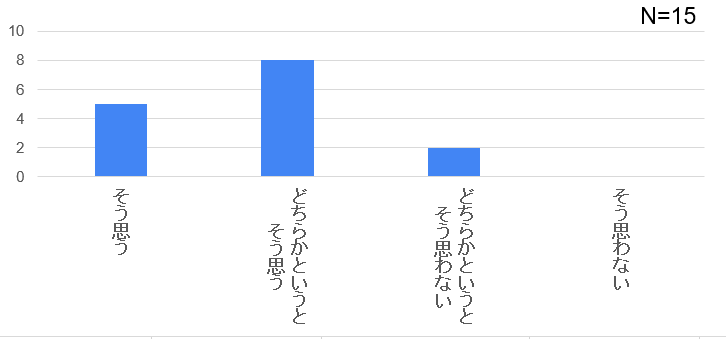
\includegraphics[width=0.7\textwidth]{fig/tab2.png}
\end{table}

また,``このbotを使うことで大規模言語モデル(ChatGPTなど)の使い方を新しく学ぶことができましたか?''の質問については同様の方法で平均を求めた結果,3.47となった.

\begin{table}[H]
    \centering
    \caption{このbotを使うことで大規模言語モデル(ChatGPTなど)の使い方を新しく学ぶことができましたか?}
    \label{tab:answer2}
    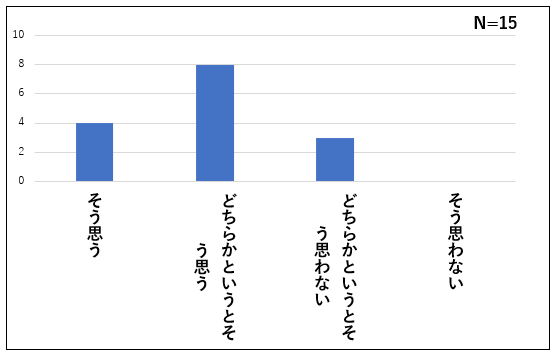
\includegraphics[width=0.7\textwidth]{fig/tab3.png}
\end{table}

そう思う~そう思わないの4段階の同じ指標で回答してもらった結果,表\ref{tab:answer2}の結果のみ平均3.47と高かったことから,botによって大規模言語モデルの新しい使い方を学べたことが示唆された.




